\chapter{Elementmetoden}

Elementmetoden (\glsentrysymbol{fem}) er en numerisk metode for å løse \gls{pde} ved å diskretisere domenet i enkle geometriske former (elementer) og tilnærme løsningen med en lineærkombinasjon av basisfunksjoner.

\begin{equation}
  u(x) \approx \sum_{i=1}^N c_i \phi_i(x)
\end{equation}

\paragraph{Betingelser}

For å bruke elementmetoden (\glsentrysymbol{fem}) til å løse et \gls{pde}-problem, må problemet oppfylle følgende betingelser:

\begin{itemize}
  \item \textbf{Linearitet:} Problemet må være lineært, dvs. ligningene kan uttrykkes som \(\mathcal{L}(u) = f\), hvor \(\mathcal{L}\) er en lineær operator.
  \item \textbf{Kontinuerlig Differensierbar:} Løsningen \( u(x) \) må være kontinuerlig differensierbar i området \( \Omega \).
  \item \textbf{Geometrisk Enkel:} Området \( \Omega \) bør kunne deles opp i enkle geometriske elementer (f.eks. trekanter, firkanter i 2D, tetraedre i 3D):
        \[
          \Omega = \bigcup_{e=1}^{E} \Omega_e
        \]
        \begin{example}{}{}
          En sirkel kan deles opp i trekanter.
          \[
            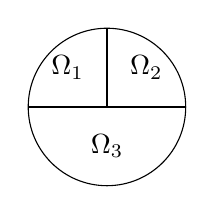
\begin{tikzpicture}
              \draw (0,0) circle (1);
              \draw (0,0) -- (1,0);
              \draw (0,0) -- (0,1);
              \draw (0,0) -- (-1,0);

              % Label the elements (triangles)
              \node at (-0.5,0.5) {\(\Omega_1\)};
              \node at (0.5,0.5) {\(\Omega_2\)};
              \node at (0,-0.5) {\(\Omega_3\)};
            \end{tikzpicture}
          \]
        \end{example}

  \item \textbf{Kvantiserbarhet:} Problemet må være kvantiserbart, dvs. løsningen kan tilnærmes med en lineærkombinasjon av basisfunksjoner:
        \[
          u_h(x) = \sum_{i=1}^{N} c_i \phi_i(x)
        \]
  \item \textbf{Randbetingelser:} Randbetingelsene må være spesifisert.
        \begin{itemize}
          \item Dirichlet: \( u(x) = \alpha \) på \(\partial \Omega_D \)
          \item Neumann: \( \frac{\partial u}{\partial n} = \beta \) på \(\partial \Omega_N \)
        \end{itemize}
\end{itemize}

\section{Generell fremgangsmåte}

\begin{enumerate}
  \item \textbf{Definer problemet:} Finn \gls{pde} og randbetingelser \(\implies\) bestem \(f(x)\) og \(\Omega\).
  \item \textbf{Diskretiser domenet:} Del opp \(\Omega\) i enkle geometriske elementer.
  \item \textbf{Lokal approksimering for hvert element:} Innenfor hvert element (ukjente området/løsning) tilnærmer vi løsningen med en lineærkombinasjon av basisfunksjoner.
        \[
          u(x) \approx \sum_{i=1}^N c_i \phi_i(x)
        \]
  \item \textbf{Svak formulering:} Formuler problemet som en \gls{weakformulation} av \gls{pde}.
        \[
          \int_\Omega v(x) \mathcal{L}(u(x)) \, dx = \int_\Omega v(x) f(x) \, dx
        \]
  \item \textbf{Formuler elementeneligningene:} Sett sammen elementene til et system av ligninger, ved å bruke \gls{weakformulation} av \gls{pde}.
        \[
          \symbf{K} \symbf{u} = \symbf{F}
        \]
  \item \textbf{Randbetingelser:} Sett opp ligningssystemet med randbetingelser.
  \item \textbf{Løs ligningssystemet:} Løs ligningssystemet for å finne koeffisientene \(u_i\).
        \[
          \symbf{u} = \symbf{K}^{-1} \symbf{F}
        \]
\end{enumerate}

\begin{example}{Poisson-ligningen}{poisson}
  \begin{equation}
    \begin{cases}
      -\ddn[2]{u(x)}{x} = f(x),         & x \in (0,1)              \\
      u(0) = \alpha, \quad u(1) = \beta & \text{(randbetingelser)}
    \end{cases}
  \end{equation}

  \begin{equation}
    \mathbf{F} = - \int_0^1 f(x) \mathbf{N}(x) dx
  \end{equation}

  La \(f(x) = \bar{f}\) være konstant. Vi antar at \(u(x_m)\) er ukjent for \(m = 1, \ldots, M\) punkter (noder) i det diskrete domenet \(\Omega_h\).

  I mellom nodene definerer vi \textit{elementene} \(\implies\) \textit{formfunksjoner} \(N_i(x)\).

  \begin{figure}[H]
    \centering
    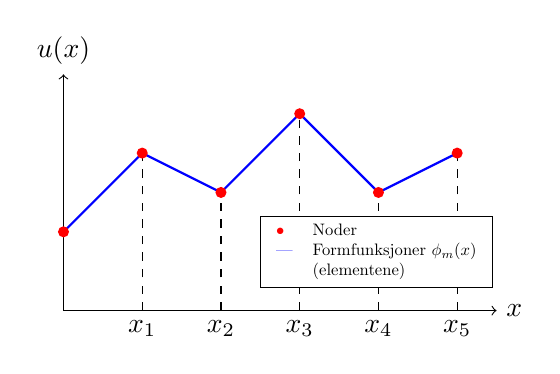
\begin{tikzpicture}
      % Coordinate axes
      \draw[->] (0,0) -- (0,3) node[above] {\(u(x)\)};
      \draw[->] (0,0) -- (5.5,0) node[right] {\(x\)};

      % Solution curve
      \draw[thick, blue] (0,1) -- (1,2) -- (2,1.5) -- (3,2.5) -- (4,1.5) -- (5,2);

      % Vertical lines at nodes with labels
      \draw[dashed] (1,0) node[below] {\(x_1\)} -- (1,2);
      \draw[dashed] (2,0) node[below] {\(x_2\)} -- (2,1.5);
      \draw[dashed] (3,0) node[below] {\(x_3\)} -- (3,2.5);
      \draw[dashed] (4,0) node[below] {\(x_4\)} -- (4,1.5);
      \draw[dashed] (5,0) node[below] {\(x_5\)} -- (5,2);

      % Nodes (intersection points)
      \fill[red] (0,1) circle (2pt);
      \fill[red] (1,2) circle (2pt);
      \fill[red] (2,1.5) circle (2pt);
      \fill[red] (3,2.5) circle (2pt);
      \fill[red] (4,1.5) circle (2pt);
      \fill[red] (5,2) circle (2pt);

      % Add legend
      \node[draw, anchor=north west, scale=0.6,fill=white] at (2.5,1.2) {
        \begin{tabular}{ll}
          \textcolor{red}{$\bullet$} & Noder                        \\
          \textcolor{blue}{---}      & Formfunksjoner \(\phi_m(x)\) \\
                                     & (elementene)                 \\
        \end{tabular}
      };
    \end{tikzpicture}
    \caption{Tilfeldig valgt formfunksjoner \(N_i(x)\) mellom nodene \(x_i\).}
  \end{figure}
  Definerer formfunksjonene som:
  \[
    \phi_i(x) = \begin{cases}
      1 - 2|x - x_i|, & |x - x_i| < 0.5 \\
      0,              & \text{ellers}
    \end{cases}
  \]
  Og testfunksjonene som:
  \[
    v(x) = \sum_{j=1}^n v_j \phi_j(x) = \symbf{v}^T \symbf{\phi}(x)
  \]

  Den svake formuleringen blir:
  \begin{align*}
    \int_0^1 \left( \sum_{j=1}^n v_j \phi_j'(x) \right)
    \left( \sum_{i=1}^n u_i \phi_i'(x) \right) \, dx
                        & =
    \int_0^1 \left( \sum_{j=1}^n v_j \phi_j(x) \right) f(x) \, dx \\
    \symbf{v}^T \, \int_0^1 \symbf{\phi}' \symbf{\phi}'^T \, dx \, \symbf{u}
                        & =
    \symbf{v}^T \int_0^1 - f(x) \symbf{\phi}  \, dx               \\
    \symbf{v}^T \symbf{K} \symbf{u}
                        & =
    \symbf{v}^T \symbf{F}                                         \\
    \symbf{K} \symbf{u} & = \symbf{F}
  \end{align*}

  Hvor:

  \begin{align*}
    \symbf{K} &= \int_0^1 \symbf{\phi}' \symbf{\phi}'^T \, dx = 
    \begin{bmatrix}
      1 & -1 & 0 & 0 & 0 & 0 \\
      -1 & 2 & -1 & 0 & 0 & 0 \\
      0 & -1 & 2 & -1 & 0 & 0 \\
      0 & 0 & -1 & 2 & -1 & 0 \\
      0 & 0 & 0 & -1 & 2 & -1 \\
      0 & 0 & 0 & 0 & -1 & 1 \\
    \end{bmatrix}\\
    \symbf{F} &= - \bar{f} \int_0^1 \symbf{N}(x) dx
    = - \bar{f}
    \begin{bmatrix}
      0.1 \\ 0.2 \\ 0.2 \\ 0.2 \\ 0.2 \\ 0.1
    \end{bmatrix}
  \end{align*}

  Løser ligningssystemet for å finne koeffisientene \(u_i\):
  \[
    \symbf{u} = \symbf{K}^{-1} \symbf{F}
  \]

\end{example}

\section{Basisfunksjoner (Formfunksjoner)}

Basisfunksjoner er byggesteinene i \gls{fem}-metoden.
De er enkle funksjoner som gjør at vi kan representere en komplisert funksjon ved hjelp av enkle byggesteiner.

\subparagraph{\gls{basisfunction}}
En \gls{basisfunction} $\phi_i(x)$ er en lokal funksjon som:
\begin{itemize}
  \item Er null overalt unntatt i nærheten av node \(i\) (lokalt definert).
  \item Har verdien 1 i node \(i\) og 0 i alle andre noder
  \item Til sammen kan bygge opp løsningen vår \(u(x)\) som en sum:
        \[
          u(x) = \sum_{i=1}^n u_i \phi_i(x) = \symbf{u}^T \symbf{\phi}(x)
        \]
  \item \(u_i\) er koeffisientene som bestemmer hvor mye av hver \gls{basisfunction} som skal brukes.
\end{itemize}


\subsection{Stykkvis lineære basisfunksjoner}

La \(u(x)\) være en tilnærming til løsningen av et \gls{pde}, og la \(u(x)\) være gitt ved en lineærkombinasjon av \gls{basisfunction}er:
\[
  u(x) = \sum_{i=1}^6 u_i N_i(x)
\]


\begin{figure}[H]
  \centering
  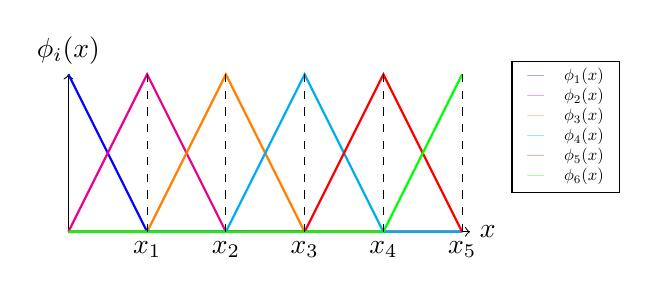
\begin{tikzpicture}
    % Coordinate axes
    \draw[->] (0,0) -- (0,2) node[above] {\(\phi_i(x)\)};
    \draw[->] (0,0) -- (5.1,0) node[right] {\(x\)};

    % Solution curve
    \draw[thick, blue] (0,2) -- (1,0) -- (5,0);
    \draw[thick, magenta] (0,0) -- (1,2) -- (2,0) -- (5,0);
    \draw[thick, orange] (0,0) -- (1,0) -- (2,2) -- (3,0) -- (5,0);
    \draw[thick, cyan] (0,0) -- (2,0) -- (3,2) -- (4,0) -- (5,0);
    \draw[thick, red] (0,0) -- (3,0) -- (4,2) -- (5,0);
    \draw[thick, green] (0,0) -- (4,0) -- (5,2);

    % Vertical lines at nodes with labels
    \draw[dashed] (1,0) node[below] {\(x_1\)} -- (1,2);
    \draw[dashed] (2,0) node[below] {\(x_2\)} -- (2,2);
    \draw[dashed] (3,0) node[below] {\(x_3\)} -- (3,2);
    \draw[dashed] (4,0) node[below] {\(x_4\)} -- (4,2);
    \draw[dashed] (5,0) node[below] {\(x_5\)} -- (5,2);

    % Legend
    \node[draw, anchor=south east, scale=0.6,fill=white] at (7,0.5) {
      \begin{tabular}{ll}
        \textcolor{blue}{---}    & \(\phi_1(x)\) \\
        \textcolor{magenta}{---} & \(\phi_2(x)\) \\
        \textcolor{orange}{---}  & \(\phi_3(x)\) \\
        \textcolor{cyan}{---}    & \(\phi_4(x)\) \\
        \textcolor{red}{---}     & \(\phi_5(x)\) \\
        \textcolor{green}{---}   & \(\phi_6(x)\) \\
      \end{tabular}
    };

  \end{tikzpicture}
  \caption{Piecewise Linear Basis Functions $\phi_i(x)$}
\end{figure}

\section{Svak formulering}
\subsubsection{Sterk formulering av PDE}
Her skriver vi \gls{pde}-en direkte i differensialform. Det betyr at vi forutsetter at løsningen u er glatt nok til at alle deriverte eksisterer. Da har vi:
\[
  \mathcal{L}(u) = f,
\]
samt presise krav på grenseverdier, for eksempel:
\[
  u|_{\partial \Omega} = g \quad \text{eller} \quad \frac{\partial u}{\partial n}\bigg|_{\partial \Omega} = h.
\]

\subsubsection{\gls{weakformulation} av PDE}
Hvis løsningen u ikke er glatt nok, bruker vi en \gls{weakformulation} av problemet.
Her tester vi u med en \gls{testfunction} \(v(x)\) over hele domenet:
\[
  \int_\Omega v^{(k)}(x) \, \mathcal{L}(u(x)) \, dx = \int_\Omega v(x) \, f(x) \, dx.
\]
Denne metoden gjør det mulig å finne løsninger i et bredere funksjonsrom.

\gls{testfunction}en er en vilkårlig funksjon som tilfredsstiller randbetingelsene.

\gls{testfunction}en velges ofte til det samme som \gls{basisfunction}en.
\[
  v(x) = \sum_{j=1}^n v_j \phi_j(x) = \symbf{v}^T \symbf{\phi}(x)
\]

\subparagraph{\gls{weakformulation} av Poisson-ligningen}
La oss se på Poisson-ligningen:
\[
  -u''(x) = f(x), \quad x \in (0,1),
\]
med randbetingelser:
\[
  u(0) = \alpha, \quad u(1) = \beta.
\]
Vi kan skrive den svake formuleringen som:
\[
  \int_0^1 v'(x) u'(x) \, dx = \int_0^1 v(x) f(x) \, dx,
\]
Velger \gls{basisfunction}er til å være:
\[
  \phi_i(x) = \begin{cases}
    1 - 2|x - x_i|, & |x - x_i| < 0.5 \\
    0,              & \text{ellers}
  \end{cases}
\]
Med \gls{testfunction}ene \(v(x) = \sum_{j=1}^n v_j \phi_j(x)\).

Da får vi:

\begin{align*}
  \int_0^1 \left( \sum_{j=1}^n v_j \phi_j'(x) \right)
  \left( \sum_{i=1}^n u_i \phi_i'(x) \right) \, dx
                      & =
  \int_0^1 \left( \sum_{j=1}^n v_j \phi_j(x) \right) f(x) \, dx \\
  \symbf{v}^T \, \int_0^1 \symbf{\phi}' \symbf{\phi}'^T \, dx \, \symbf{u}
                      & =
  \symbf{v}^T \int_0^1 - f(x) \symbf{\phi}  \, dx               \\
  \symbf{v}^T \symbf{K} \symbf{u}
                      & =
  \symbf{v}^T \symbf{F}                                         \\
  \symbf{K} \symbf{u} & = \symbf{F}
\end{align*}



